%%%%%%%%%%%%%%%%%%%%%%%%%%%
\chapter {Introduction}
\label{INTRO}
%%%%%%%%%%%%%%%%%%%%%%%%%%%

  A distributed system is a group of computational entities cooperating with each to achieve one or more tasks. This thesis deals with distributed computing by mobile agents in network. More specifically, we deal with the problem of deploying a group of mobile agents who follow the same protocol to explore the network and decontaminate the dangerous virus (called Black Virus) present on the network nodes.
  In this chapter, the motivations of the problem are provided, following is a brief summary of the contributions.Finally, an overview of the organization of the thesis is presented.


\section{Problem and Motivation} 
Mobile agents are widely used in distributed and network systems while the applications of them can cause some security issues, thus threatening to the network: A contaminated or infected host can destroy working agents for various malicious purposes; A malicious agent can contaminate or infect other computer nodes so they become malfunctional or crash.
  The harmful hosts, often called {\em Black Holes} trigger the problem called {\em Black Hole Search} (BHS), the focus of which is to locate their positions since it is statics. This problem has been studied in many variants. For example, different topologies and different settings (synchronous and asynchronous). The harmful agents trigger the problem called {\em Intruder Capture} (IC). Its main focus is to deploy a group of mobile agents to capture a extraneous mobile agent (the intruder) who moves arbitrarily fast through the network and infects the visiting sites. Also it has been investigated in a variety of topologies. More detailed literature review will be provided in Chapter 2. Note that BH is static and only damage the agents reaching it without leaving any detectable trace. Intruder is mobile and harmful to the network nodes but does not cost any harm to other system agents. 
    A new harmful presence called {\em black virus} BV has been initially introduced by Cai et al. in\cite{Cai}. It is a dangerous process resides at an unknown site in a network and destroys any upcoming agents, but unlike the BH, the node where the original BV resides thus become clean. At the same time, the original BV multiplies (called clones) and spread to all neighbouring nodes, thus increasing its number,and damage in the network. A BV is destroyed when it moves to a site where there is already an agent. Based on this harmful presence, a new problem called Black Virus Decontamination(BVD) is presented by Cai et al., the main focus of which is to use a group of system agents to permanently remove any presence of the BV from the network. A protocol defining the actions of the agents solves the BVD problem if at least one agent survives and the network is free of BVs. Also, a desirable property of a  decontamination protocol is that the nodes which have been explored or cleaned by mobile agents are not be recontaminated by the BV spreading. A solution protocol with such a property will be called {\em monotone}. see\cite{monotone}.
Some important cost measure is the number of node infections by the BVs (casualties); size of the team, i.e, the number of agents employed by the solution, the time needed by the solution. 
    Solutions in which the agents explore the network's node in sequence have been proposed in \cite{Cai}, \cite{Alotaibi} and \cite{ Cai1}. The size of team is minimum in \cite{Cai} and the number of site infections is also minimum in such case,i.ie., exploring the network nodes in sequence. Now we are interested in the solution using parallel strategy where we deploy a larger number of mobile agents following the same protocol to decontaminate the network in the exploring phase with the goal to minimize the {\em total working time} (TWT) which is caculated by multiplying the number of agents and the total execution time and also the casualties.


%---------------------------------
\section{Our Contribution} 


\begin{enumerate}
\item In this thesis, we propose parallel strategy to solve the BVD problem. It is the first attempt to deal with this issue in a parallel way. Agents are not allowed to communicate with each other unless they are in the same network node so the protocol should enable the agents in different nodes to move properly, i.e, the route of every agent is different but they are served to explore the network; when a BV is triggered, other agents should bypass the new-formed BVs... We give simple but efficient solution to deal with this problem with acceptable cost. Also we give the size of the exploring team which is minimum to guarantee both the TWT and the  casualties we reach.
\item The BVD problem is investigated for three important topologies: {\em meshes}, {\em tori}, {\em chordal rings}. All the protocol are optimal both in term of TWT and casualties. We compare our solution with \cite{Cai} and \cite{Alotaibi} in which the exploring route is in sequence and the result is that our solution is better than that of them in both TWT and casualties. One should be point out that in chordal ring especially, the more complicated the chordal ring becomes, the more TWT that we save comparing to \cite{Alotaibi}.
\end{enumerate}

%---------------------------------

\section{Thesis Organization} 

The thesis is organized as followed:

Chapter 2 contains a literature review on related problems. We begin by reviewing the Black Hole Search and Intruder Capture problem, and then focus on the solution of BVD problem where the mobile agents explore the network in sequence, the issue has been studies in different topologies: two-dimensional grids, three-dimensional grids, tori, chordal rings, hypercubes and arbitrary network. Also, the variant of this problem, which is decontamination of an arbitrary network from multiple black virus is also reviewed. We also present our assumption and the topologies ( meshes, tori, chordal rings).

Chapter 3 introduces terminology, definitions and model for the BVD problem used in the rest of the thesis. Also we describe the high level ideas that serve as the basic of all our solutions. Since monontone is the necessary condition for spread optimality, we go through the principle and finally make a conclusion.

Chapter 4 focus on the BVD problem for two simple classes of network topologies: {\em meshes} and {\em tori}. For each kind of network, an optimal algorithm in terms of casualties and TWT is developed. Complexity analysis in terms of casualty and TWT are performed and obtained. Some comparison and analysis are also made between our solution and \cite{Cai} and the result shows that our solution is better.

Chapter 5 presents the BVD problem for the chordal ring topology. In this chapter, we introduce the {\em Three Jump Notifying Technique} (TJNT) to manipulate each mobile agent efficiently go through their route in the exploring phase and avoid any new-formed BV after the original BV is triggered. Based on this technique, we develop the parallel strategy for the mobile agents to decontaminate the choral ring from BV. Complexity analysis in terms of  casualty and TWT are performed. Finally some comparison and analysis are made between our solution and \cite{Alotaibi} and the result shows that our solution performs better.

Chapter 6 summaries the main conclusion of our work and present some open problems and future work.
  



\begin{comment}


\begin{figure}[H]
  \centering  
  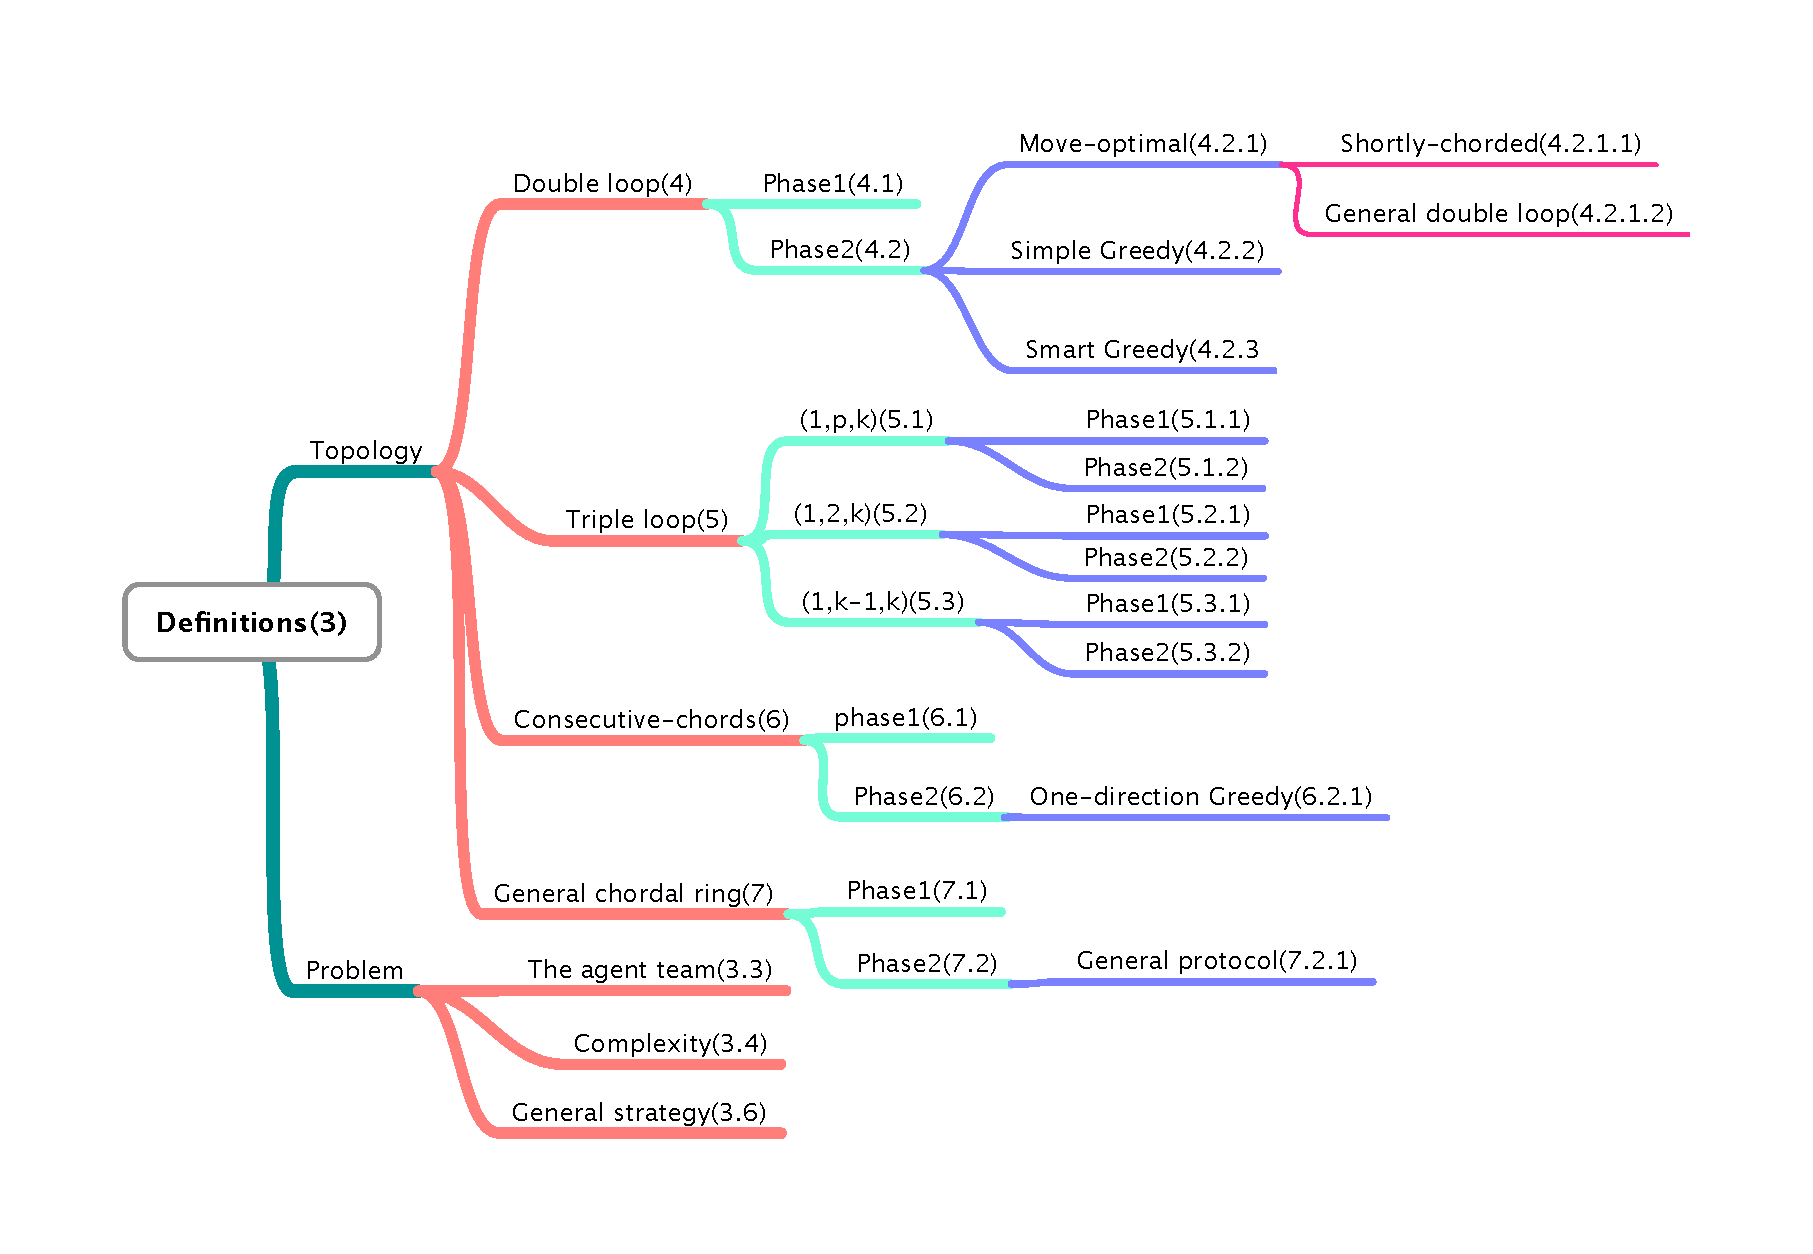
\includegraphics[width=1\textwidth]{figures/map2.pdf}
  \caption{A map showing the organization of the thesis}
\end{figure}

\end{comment}
